\documentclass[10pt]{article}
\usepackage[usenames]{color} %used for font color
\usepackage{amssymb} %maths
\usepackage{fancyvrb}
\usepackage{amsmath} %maths
\usepackage[utf8]{inputenc} %useful to type directly diacritic characters
\usepackage[letterpaper, portrait, margin=1in]{geometry}
\usepackage{graphicx,wrapfig}
\usepackage{booktabs}
\usepackage{multicol}
\begin{document}
\subsection*{MSDS650 Week 6 Python  Assignment - Nathan Worsham}
I work with Linux day in and day out and most of the Linux commands I am already familiar with so I felt it made more sense to continue working with my Python skills. I worked through the Python tutorial with no issues. I felt it made more sense however to use the code as script rather than work with it on the IDLE. To do this I made the code the author created into a function and commented out the folder variable line and changed the \verb|f| variable line to instead read a variable called \verb|file| which would be fed to the function. Then in the main function area I grabbed the first system argument--\verb|sys.argv[1]|--as the input file and called the previous function with the input file as an argument. This way it made it very simple to feed the script any book.
Trying to install matplotlib on OSX, I received an error that it couldn't be installed that it required "System Python" 2.7. To get around this I used homebrew to install Python using the instructions from this site--http://docs.python-guide.org/en/latest/starting/install/osx/. I then used pip to install matplotlib, which did install the matplotlib version that was not recommended (the 64bit). But I decided to try to go with it anyway, and the exercise did work on my system and produced the graph as expected. 
Next for choosing a book, I decided to go with the book of Isaiah from the old testament. When you search for a text version of the Bible, you can only seem to find the King James version. I didn't want to deal with old colloquialisms like 'ye', so I ended up finding the "Basic English Version". The version I found placed each book in its own folder with each chapter in a separate text file. So to combine these into one file I used this command from inside the Isaiah folder:
\begin{verbatim}
cat * > Isaiah.txt
\end{verbatim}
Now I had a file I could easily feed to the script. On the first pass I received the following results:
%\begin{wrapfigure}{r}{5cm}
%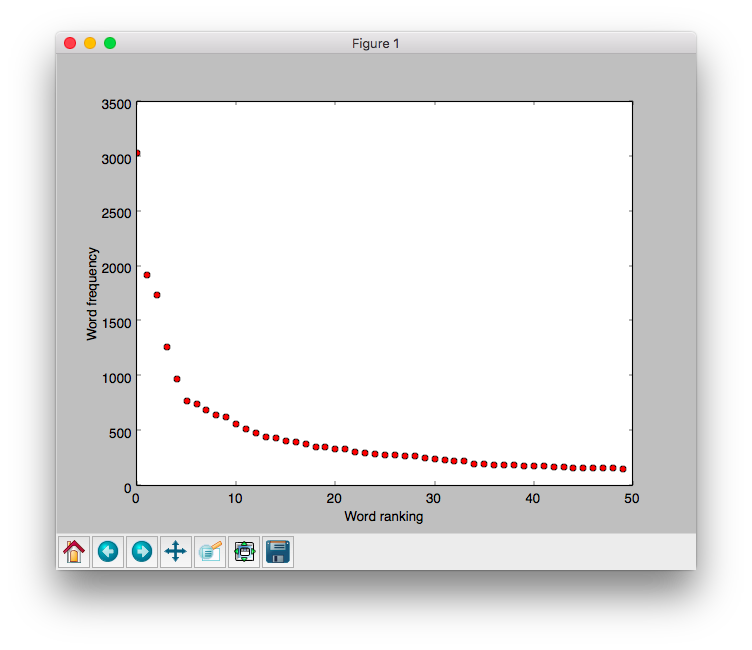
\includegraphics[width=5cm, scale=0.2]{Isaiah_graph1.png}
%\end{wrapfigure}
\begin{Verbatim}[fontsize=\small]
b18608:week6 worshamn$ ./week6.py Isaiah.txt 
Run took  0.0490620136261  seconds.
Number of distinct words:  1847
\end{Verbatim}
\begin{multicols}{2}
\begin{Verbatim}[fontsize=\small]
('the', 3026)
('and', 1915)
('of', 1736)
('will', 1254)
('to', 962)
('in', 762)
('be', 742)
('for', 686)
('a', 636)
('you', 619)
('is', 560)
('your', 508)
('lord', 471)
('i', 440)
('have', 429)
('who', 404)
('his', 391)
('my', 370)
('are', 350)
('it', 342)
('on', 324)
('he', 324)
('not', 302)
('their', 296)
('come', 278)
('give', 275)
('they', 271)
('from', 265)
('with', 263)
('no', 248)
('has', 241)
('all', 232)
('make', 221)
('that', 220)
('up', 194)
('them', 188)
('put', 184)
('like', 183)
('me', 179)
('him', 171)
('by', 171)
('out', 169)
('go', 161)
('made', 160)
('those', 156)
('but', 156)
('as', 155)
('this', 154)
('there', 151)
('let', 142)
\end{Verbatim}
\end{multicols}
\pagebreak
\begin{figure}[!h]
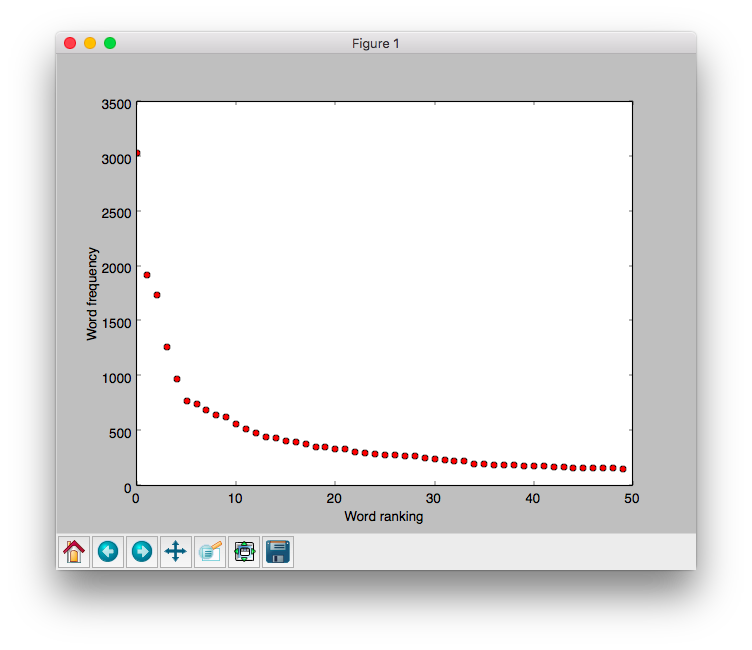
\includegraphics[scale=0.37]{Isaiah_graph1.png}
\centering
\end{figure}
Looking at the results, I find from last week's exercise that many of the words are "stop words". So next I decided to edit the code some more and deal with stop words. The most thorough stop word list I could find for the English language was from Michael Ecklund (2012), which was a list of 758 words. So placing that in a file in the same directory, each line of the file was one word, I then added some new lines to read the stop word file and remove the word from the "huck" dictionary if it is one of the stop words. This drastically changed the results:
\begin{Verbatim}[fontsize=\small]
b18608:week6 worshamn$ ./week6.py Isaiah.txt stopwords_2.csv 
Run took  0.0859479904175  seconds.
Number of distinct words:  1581
\end{Verbatim}
\begin{multicols}{2}
\begin{Verbatim}[fontsize=\small]
('lord', 471)
('people', 130)
('god', 127)
('earth', 122)
('land', 109)
('day', 94)
('israel', 93)
('man', 92)
('waste', 89)
('word', 88)
('place', 87)
('men', 81)
('holy', 76)
('fear', 75)
('strong', 73)
('glory', 69)
('hand', 67)
('1', 66)
('2', 66)
('3', 66)
('4', 66)
('5', 66)
('6', 66)
('armies', 64)
('7', 63)
('8', 62)
('king', 61)
('9', 61)
('evil', 59)
('10', 59)
('11', 58)
('food', 58)
('knowledge', 57)
('12', 56)
('nations', 55)
('ear', 54)
('eyes', 51)
('13', 51)
('destruction', 50)
('jerusalem', 49)
('broken', 48)
('send', 48)
('14', 47)
('turned', 47)
('town', 47)
('righteousness', 47)
('house', 46)
('great', 46)
('zion', 45)
('jacob', 44)
\end{Verbatim}
\end{multicols}
\begin{figure}[!h]
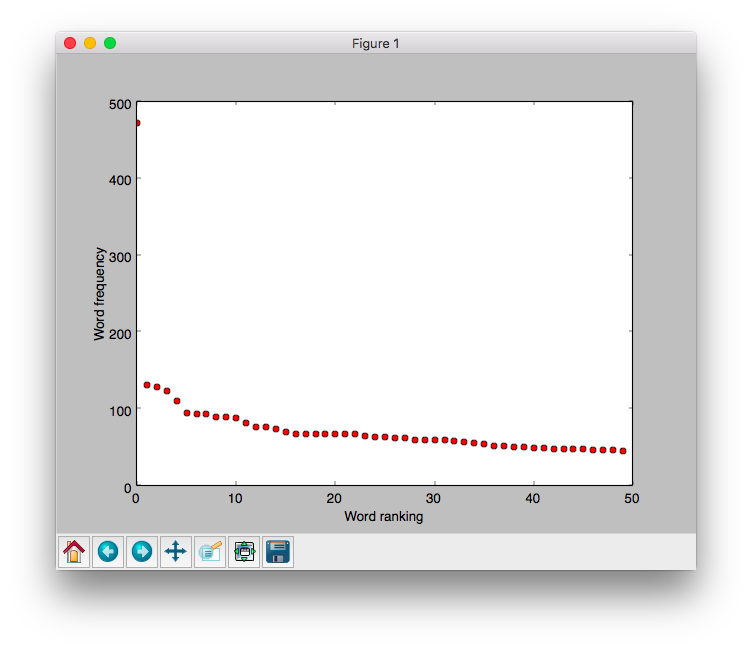
\includegraphics[scale=0.37]{Isaiah_graph2.png}
\centering
\end{figure}
Now I was running into an issue which was verse numbers were causing incorrect results--each line is a verse in this file, starting with the verse number. So I added this line to remove the numbers from the beginning of each line inserted before the line is split into words:
\begin{verbatim}
line = re.sub('^\d+\s','',line)
\end{verbatim}
Running the results this time, now looked like much more intelligent results and the resulting graph (compared to the first) having a smoother curve. We now have 1543 distinct words instead of 1581. The top word by far--Lord--but the other words definitely correspond with the themes of Isaiah being a very prophetic and apocalyptic book, such as destruction, righteousness, wrath, and salvation. Wanting to see how this compared with another old testament book. I first chose Ecclesiastes, but it is a shorter book and only has 442 distinct words, so instead I used the book of Psalms. Psalms had a closer distinct count of words at 1333 but seemingly higher count of words in general.
\par
\raisebox{-.5\height}{
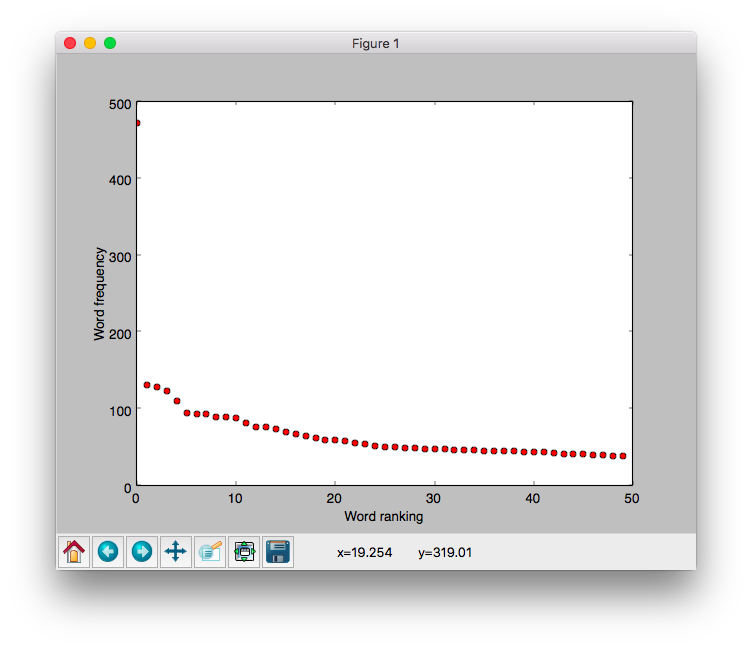
\includegraphics[width=6cm]{Isaiah_graph3.png}
}%
\hfill
\raisebox{-.5\height}{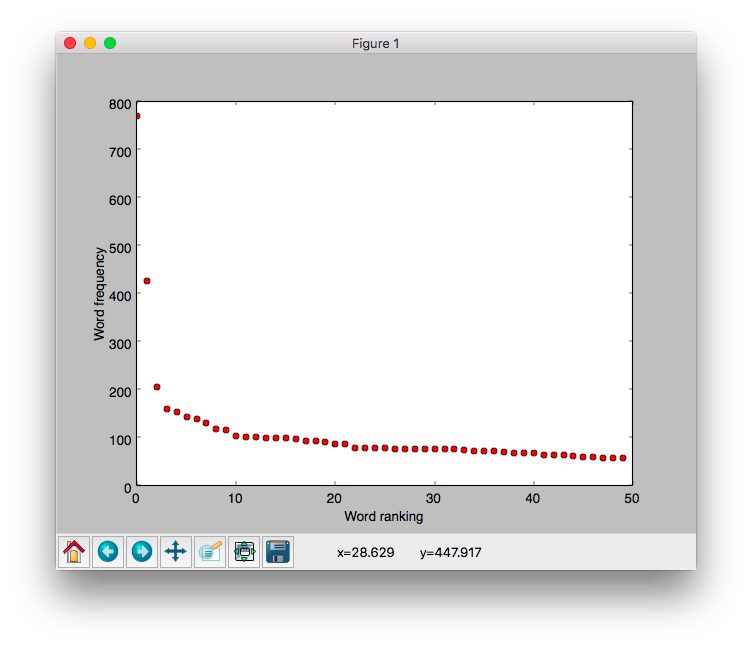
\includegraphics[width=6cm]{Psalms_graph.png}}%
\par
\pagebreak
\begin{multicols}{2}
Isaiah
\begin{Verbatim}[fontsize=\scriptsize]
('lord', 471)
('people', 130)
('god', 127)
('earth', 122)
('land', 109)
('day', 94)
('israel', 93)
('man', 92)
('waste', 89)
('word', 88)
('place', 87)
('men', 81)
('holy', 76)
('fear', 75)
('strong', 73)
('glory', 69)
('hand', 67)
('armies', 64)
('king', 61)
('evil', 59)
('food', 58)
('knowledge', 57)
('nations', 55)
('ear', 54)
('eyes', 51)
('destruction', 50)
('jerusalem', 49)
('broken', 48)
('send', 48)
('turned', 47)
('town', 47)
('righteousness', 47)
('house', 46)
('great', 46)
('zion', 45)
('jacob', 44)
('dry', 44)
('egypt', 44)
('joy', 44)
('wrath', 43)
('heart', 43)
('high', 43)
('salvation', 42)
('punishment', 41)
('children', 41)
('places', 40)
('gave', 39)
('light', 39)
('voice', 38)
('rest', 38)
\end{Verbatim}
Psalms
\begin{Verbatim}[fontsize=\scriptsize]
('lord', 768)
('god', 424)
('praise', 205)
('earth', 159)
('mercy', 152)
('great', 141)
('man', 137)
('evil', 129)
('soul', 116)
('heart', 114)
('people', 103)
('salvation', 101)
('faith', 101)
('men', 98)
('good', 98)
('righteousness', 98)
('word', 96)
('hand', 92)
('turned', 92)
('place', 90)
('strength', 86)
('haters', 86)
('upright', 78)
('eyes', 77)
('hands', 77)
('fear', 77)
('gave', 76)
('glad', 76)
('glory', 76)
('holy', 75)
('high', 75)
('life', 74)
('words', 74)
('unchanging', 73)
('day', 71)
('selah', 70)
('voice', 70)
('land', 69)
('knowledge', 67)
('trouble', 66)
('joy', 66)
('nations', 63)
('strong', 63)
('house', 62)
('power', 60)
('israel', 59)
('children', 58)
('prayer', 57)
('song', 57)
('chief', 57)
\end{Verbatim}
\end{multicols}
The two books do look very comparable with the types of words that show up, in fact there are 31 words in common. They are: children, day, earth, evil, eyes, fear, gave, glory, god, great, hand, heart, high, holy, house, israel, joy, knowledge, land, lord, man, men, nations, people, place, righteousness, salvation, strong, turned, voice, word. I suppose I used a mixture of both assignments to find this out using Linux tools (albeit on Mac OSX) by first copying and pasting the top 50 words for each into separate files and then using these commands:
\begin{verbatim}
cat Isaiah50 |cut -d ',' -f 1 |cut -d "'" -f 2 |sort > Isaiah50.txt
cat Psalms50 |cut -d ',' -f 1 |cut -d "'" -f 2 |sort > Psalms50.txt 
comm -1 -2 Isaiah50.txt Psalms50.txt  #for the list of common words
comm -1 -2 Isaiah50.txt Psalms50.txt | wc -l #for the count of common words
\end{verbatim}
Though there are 31 words in common of the top 50 words, they are of course in different proportion within each book. But the words Lord, God, and Earth are important to each book with each book sharing Lord as the top word.
\pagebreak
\subsection*{References}
Reitz, Kenneth. 2014. Retrieved from http://docs.python-guide.org/en/latest/starting/install/osx/\\
Ruwach, 2008. Retrieved from https://sites.google.com/site/ruwach/bibletext\\
Ecklund, Michael. 2012. Retrieved from http://www.michaelbrentecklund.com/blog/english-language-stop-words-list-format-php-array-format-csv-format/
\end{document}
